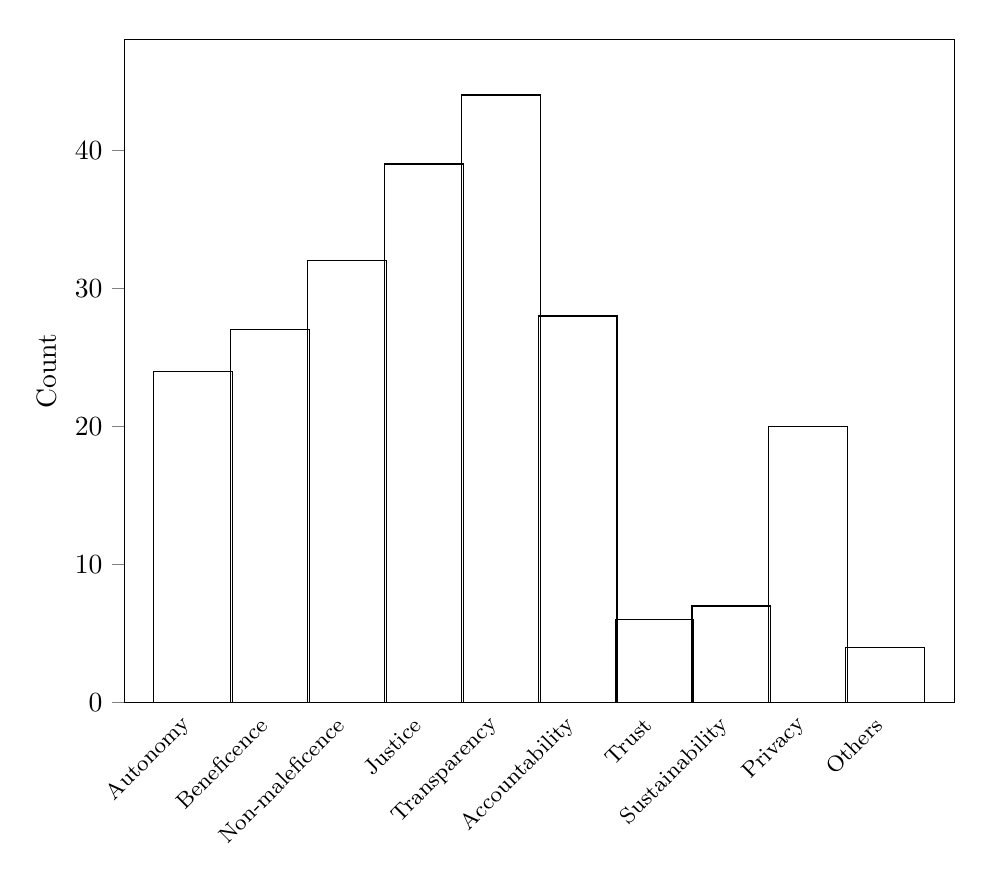
\begin{tikzpicture}
\begin{axis}[
    ybar,
    xtick=data,
    width=\textwidth,
    height = 10cm,
    bar width = 10mm,
    % enlarge x limits={abs=2cm},
    symbolic x coords={Autonomy, Beneficence, Non-maleficence, Justice, Transparency, Accountability, Trust, Sustainability, Privacy, Others},
    ylabel= Count,
    % xlabel= Principle,
    ytick align=outside,
    ytick pos=left,
    major x tick style = transparent,
    x tick label style={font=\footnotesize,rotate=45, anchor=east},
    ]
    \addplot[ybar] coordinates {
        (Autonomy,24)
        (Beneficence,27)
        (Non-maleficence,32)
        (Justice,39)
        (Transparency,44)
        (Accountability,28)
        (Trust,6)
        (Sustainability,7)
        (Privacy,20)
        (Others,4)
    };
\end{axis}
\end{tikzpicture}